\documentclass[onecolumn]{article}
%\usepackage{url}
%\usepackage{algorithmic}
\usepackage[a4paper]{geometry}
\usepackage{datetime}
\usepackage[margin=2em, font=small,labelfont=it]{caption}
\usepackage{graphicx}
\usepackage{mathpazo} % use palatino
\usepackage[scaled]{helvet} % helvetica
\usepackage{microtype}
\usepackage{amsmath}
\usepackage{subfigure}
% Letterspacing macros
\newcommand{\spacecaps}[1]{\textls[200]{\MakeUppercase{#1}}}
\newcommand{\spacesc}[1]{\textls[50]{\textsc{\MakeLowercase{#1}}}}

\title{\spacecaps{Project Report: Solving CAPTCHA's}\\ 
\normalsize \spacesc{CENG 3521, DATA MINING} }

\author{Buse Mısra TURGUT     Aylin DURAN\\
busemisraturgut@posta.mu.edu.tr   aylinduran.posta.mu.edu.tr}
%\date{\today\\\currenttime}
\date{\today}

\begin{document}
\maketitle

\begin{abstract}
CAPTCHAs are images designed to be easy for humans to solve and hard for a computer to solve, as per the acronym: Completely Automated Public Turing test to tell Computers and Humans Apart. Many websites use them for registration and commenting systems to stop automated programs flooding their site with fake accounts and spam comments.

In this project, we extracted text from images by using neural networks. The problem we are trying to solve is to automatically understand CAPTCHA messages. We worked with images in order to use simple pixel values to predict the letter being portrayed in a CAPTCHA.
\end{abstract}


\section{Introduction}
If  we  need to define neural networks simply, we can say that neural networks are a
class of algorithm that was originally designed based on the way that human brains work. A neural network is a collection of neurons that are connected together. Each neuron is a simple function of its inputs, which generates an output. The functions that define a neuron's processing can be any standard function, such as a linear combination of the inputs, and are called the activation function.\\
For data mining applications, the arrangement of neurons is usually in layers. The
first layer is the 'input layer', it takes the inputs from the dataset. The outputs of each
of these neurons are computed and then passed along to the neurons in the next
layer. The outputs of one layer become the inputs of the next layer, continues until we
reach the last layer which means the 'output layer'. Any layer between the input and output layer is called hidden layer. 


\section{Assignments}
Our CAPTCHA-breaking algorithm will make the following assumptions. First, the
word will be a whole four-character English word. Second, the word will only contain
uppercase letters. No symbols, numbers, or spaces will be used.  We are going to perform a shear transform to the text, along with varying rates of shearing.

\subsection{Assignment 1 (``Drawing Basic CAPTCHA's'')}

Our first goal is to draw an image with a word on it, along with a shear transform. We are going to use the PIL library to draw CAPTCHAs and the scikit-image library to perform the shear transform. The scikit-image library will read images in a NumPy array format that PIL can export to, allowing us to use both libraries.

\begin{figure}[h]
    \centering
    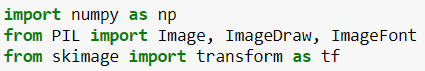
\includegraphics[width=.5\linewidth]{1..png}
\caption{\label{fig:demo-bad}
\centering
Importing.\\We install PIL and scikit-image libraries, then we import necessary libraries and modules: NumPy  and Image drawing functions}
\end{figure}

\begin{figure}[h]
    \centering
    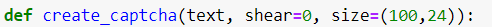
\includegraphics[width=.5\linewidth]{2..png}
\caption{\label{fig:demo-bad}
\centering
generate.\\Then we create our base function for generating CAPTCHAs. This function takes a word and a shear value (which is normally between 0 and 0.5) to return an image in a NumPy array format.}
\end{figure}

\begin{figure}[h]
    \centering
    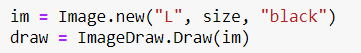
\includegraphics[width=.5\linewidth]{3..png}
\caption{\label{fig:demo-bad}
\centering
image.\\We create a new image using L for the format, which means black-and-white pixels only, and create an instance of the ImageDraw class. This allows us to draw on this
image using PIL.}
\end{figure}

\begin{figure}[hb!]
    \centering
    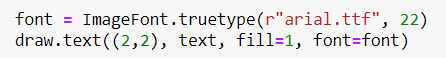
\includegraphics[width=.5\linewidth]{4..png}
\caption{\label{fig:demo-bad}
\centering
Here we set the font of the CAPTCHA we will use}
\end{figure}

\begin{figure}[hb!]
    \centering
    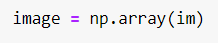
\includegraphics[width=.3\linewidth]{5..png}
\caption{\label{fig:demo-bad}
\centering
conversion.\\We convert the PIL image to a NumPy array, which allows us to use scikit-image to perform a shear on it.}
\end{figure}

\begin{figure}[hb!]
    \centering
    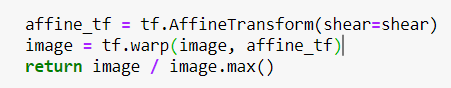
\includegraphics[width=.7\linewidth]{6..png}
\caption{\label{fig:demo-bad}
\centering
\\We then apply the shear transform and return the image. In the last line, we normalize by dividing by the maximum value, ensuring our
feature values are in the range 0 to 1.}
\end{figure}

\newpage
\begin{t}
 From here, we can now generate images quite easily and use pyplot to display them.
\end{t}



\begin{figure}[h]
    \centering
    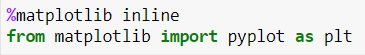
\includegraphics[width=.5\linewidth]{7..png}
\caption{\label{fig:demo-bad}
\centering
\\we use our inline display for the matplotlib graphs and import pyplot.}
\end{figure}

\begin{figure}[h]
    \centering
    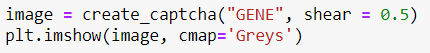
\includegraphics[width=.5\linewidth]{8..png}
\caption{\label{fig:demo-bad}
\centering
\\Then we create our first CAPTCHA and show it}
\end{figure}

\begin{figure}[h]
    \centering
    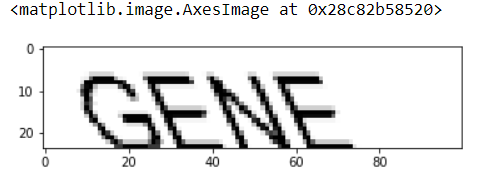
\includegraphics[width=.5\linewidth]{9..png}
\caption{\label{fig:demo-bad}
\centering
\\this is what our first CAPTCHA looks like.}
\end{figure}

\subsection{Assignment 2 (``Splitting the Image Into Individual Letters'')}
\begin{t}
Now we will break the problem down into a smaller problem: predicting letters. The next step is segmenting the word to discover each of the letters within it. To do this, we are going to create a function that finds contiguous sections of black pixels on the image and extract them as sub-images. These are going to be our letters.
\end{t}

\begin{figure}[hb!]
    \centering
    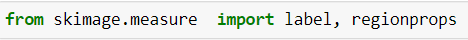
\includegraphics[width=.5\linewidth]{10..png}
\caption{\label{fig:demo-bad}
\centering
importing\\First we import the label and regionprops functions, because we will use them in our function.}
\end{figure}

\begin{figure}[hb!]
    \centering
    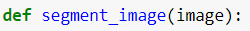
\includegraphics[width=.3\linewidth]{11..png}
\caption{\label{fig:demo-bad}
\centering
defining function\\Our function will take an image, and return a list of subimages, where each sub-image is a letter from the original word in the image.}
\end{figure}

\newpage
\begin{t}
The first thing we need to do is to detect where each letter is. To do this, we will use the label function in scikit-image, this finds connected sets of pixels that have the same value.
\end{t}

\begin{figure}[h]
    \centering
    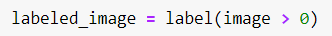
\includegraphics[width=.5\linewidth]{12..png}
\caption{\label{fig:demo-bad}
\centering
defining function\\The label function takes an image and returns an array of the same shape as the
original.}
\end{figure}

\begin{figure}[h]
    \centering
    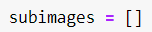
\includegraphics[width=.2\linewidth]{13..png}
\caption{\label{fig:demo-bad}
\centering
listing\\We are getting each of these sub-images and place them into a list.}
\end{figure}

\begin{figure}[h]
    \centering
    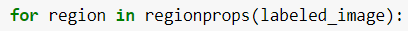
\includegraphics[width=.5\linewidth]{14..png}
\caption{\label{fig:demo-bad}
\centering
\\The scikit-image library also contains a function for extracting information about these regions. We can iterate over these regions and work on each individually.}
\end{figure}

\begin{figure}[hb!]
    \centering
    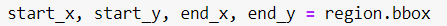
\includegraphics[width=.5\linewidth]{15..png}
\caption{\label{fig:demo-bad}
\centering
\\we can query the region object for information about the current region. For our algorithm, we need to obtain the starting and ending coordinates of the current region.}
\end{figure}

\begin{figure}[hb!]
    \centering
    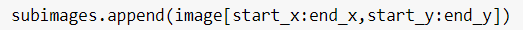
\includegraphics[width=.6\linewidth]{16..png}
\caption{\label{fig:demo-bad}
\centering
\\We can then extract the sub-images by indexing the image (it was represented as a simple NumPy array, so we can easily index it) using the starting and ending positions of the sub-image, and adding the selected sub-image to our list.}
\end{figure}

\begin{figure}[hb!]
    \centering
    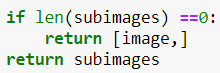
\includegraphics[width=.3\linewidth]{17..png}
\caption{\label{fig:demo-bad}
\centering
\\Finally  we return the discovered sub-images, each of them containing the section of the image with an individual letter in it. If we didn't find any sub-images, code will be returning the original image as only sub-image.}
\end{figure}

\newpage
\begin{figure}[h]
    \centering
    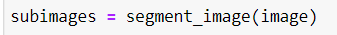
\includegraphics[width=.4\linewidth]{18..png}
\caption{\label{fig:demo-bad}
\centering
\\We can then get the sub-images from the example CAPTCHA using this function.}
\end{figure}

\begin{figure}[h]
    \centering
    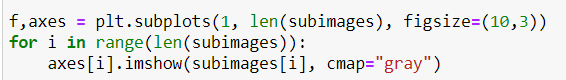
\includegraphics[width=.6\linewidth]{19..png}
\caption{\label{fig:demo-bad}
\centering
to show\\If we want to view each of these sub-images we can show them. Result looks like this:}
\end{figure}

\begin{figure}[h]
    \centering
    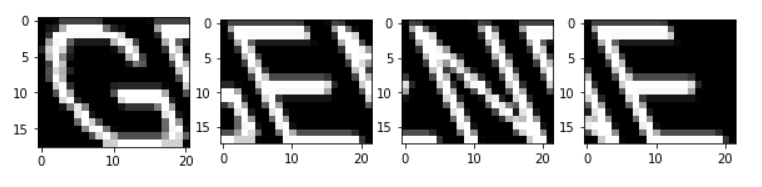
\includegraphics[width=.4\linewidth]{20..png}
\caption{\label{fig:demo-bad}
\centering
result\\As you can see in figure 20, our image segmentation does a reasonable job.}
\end{figure}

\subsection{Assignment 3 (``Creating A Training Dataset'')}
\begin{t}
Now we can create a dataset of letters, each with different shear values.
\end{t}

\begin{figure}[hb!]
    \centering
    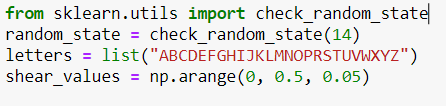
\includegraphics[width=.6\linewidth]{21..png}
\caption{\label{fig:demo-bad}
\centering
 \\We  set up our random state and an array that holds the options for letters and shear values that we will randomly select from.}
\end{figure}

\begin{figure}[hb!]
    \centering
    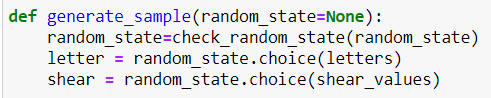
\includegraphics[width=.6\linewidth]{22..png}
\caption{\label{fig:demo-bad}
\centering
 \\We  create a function (for generating a single sample in our training dataset)
that randomly selects a letter and a shear value from the available options.}
\end{figure}

\newpage
\begin{figure}[ht]
    \centering
    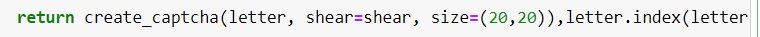
\includegraphics[width=.8\linewidth]{23..png}
\caption{\label{fig:demo-bad}ü
\centering
\\\We return the image of the letter, along with the target value representing the letter in the image.}
\end{figure}

\begin{figure}[h]
    \centering
    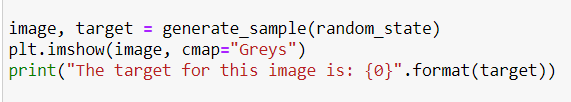
\includegraphics[width=.8\linewidth]{24..png}
\caption{\label{fig:demo-bad}
\centering
\\Outside the function block, we can now call this code to generate a new sample and then show it using pyplot.}
\end{figure}

\begin{figure}[h]
    \centering
    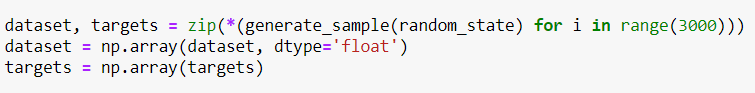
\includegraphics[width=.9\linewidth]{25..png}
\caption{\label{fig:demo-bad}
\centering
\\We can now generate all of our dataset by calling this several thousand times.
We then put the data into NumPy arrays.}
\end{figure}

\begin{figure}[hb!]
    \centering
    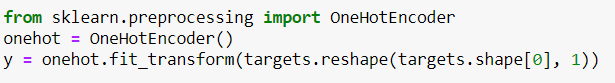
\includegraphics[width=.8\linewidth]{26..png}
\caption{\label{fig:demo-bad}
\centering
\\We perform one hot-encoding, giving us a target array that has 26 outputs per sample, using values near 1 if that letter is likely if not 0.}
\end{figure}

\begin{figure}[hb!]
    \centering
    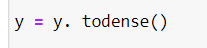
\includegraphics[width=.4\linewidth]{27..png}
\caption{\label{fig:demo-bad}
\centering
\\The library we use doesn't support sparse arrays, so we need to turn our sparse matrix into a dense NumPy array.}
\end{figure}


\newpage
\subsection{Assignment 4 (``Adjusting our training dataset to our methodology'')}

Our dataset here is nicely created individual letters, fitting the 20-pixel by 20-pixel image.
The methodology involves extracting the letters from words. we will just run our segmentation function on the training dataset and return those letters instead.

\begin{figure}[h]
    \centering
    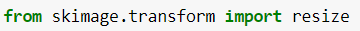
\includegraphics[width=.5\linewidth]{28..png}
\caption{\label{fig:demo-bad}
\centering
resize function\\We will need the resize function from scikit-image, as our sub-images won't
always be 20 pixels by 20 pixels.}
\end{figure}

\begin{t}
From here, we run our segment image function on each sample and then resize
them to 20 pixels by 20 pixels as it seems in figure 29.
\end{t}

\begin{figure}[h]
    \centering
    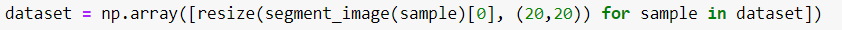
\includegraphics[width=.9\linewidth]{29..png}
\caption{\label{fig:demo-bad}
\\}
\end{figure}

\begin{t}
Finally, we will create our dataset. This dataset array is three-dimensional, as it
is an array of two-dimensional images.
\end{t} 

\begin{figure}[h]
    \centering
    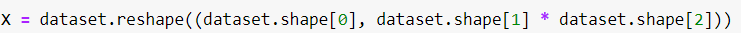
\includegraphics[width=.9\linewidth]{30..png}
\caption{\label{fig:demo-bad}
\centering
\\Our classifier will need a two-dimensional array, so we simply flatten the last two dimensions}
\end{figure}

\begin{figure}[hb!]
    \centering
    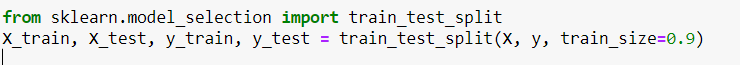
\includegraphics[width=.9\linewidth]{31..png}
\caption{\label{fig:demo-bad}
\centering
\\we create a set of data for training and one for testing.}
\end{figure}


\newpage
\subsection{Assignment 5 (``Training and Classifying'')}

\begin{t}
We are now going to build a neural network that will take an image as input and
try to predict which letter is in the image.
We will use the training set of single letters we created earlier. The dataset itself is
quite simple. We have a 20 by 20 pixel image, each pixel 1 (black) or 0 (white). These
represent the 400 features that we will use as inputs into the neural network. The
outputs will be 26 values between 0 and 1.
We are going to use the PyBrain library for our neural network.
\end{t}

\begin{figure}[hb!]
    \centering
    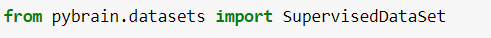
\includegraphics[width=.6\linewidth]{32..png}
\caption{\label{fig:demo-bad}
\centering
\\PyBrain library uses its own dataset format. We create training and testing datasets using this format.}
\end{figure}

\begin{figure}[h]
    \centering
    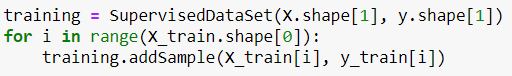
\includegraphics[width=.6\linewidth]{33..png}
\caption{\label{fig:demo-bad}
\centering
\\We iterate over our training dataset and add each as a sample into a new SupervisedDataSet instance.}
\end{figure}

\begin{figure}[h]
    \centering
    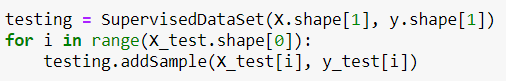
\includegraphics[width=.6\linewidth]{34..png}
\caption{\label{fig:demo-bad}
\centering
\\Here we iterate over our testing dataset and add each as a sample into a new
SupervisedDataSet instance for testing this time.}
\end{figure}


\begin{t}
Now we can build a neural network. We will create a basic three-layer network that
consists of an input layer, an output layer, and a single hidden layer between them.
The number of neurons in the input and output layers is fixed. 400 features in our
dataset dictates that we need 400 neurons in the first layer, and 26 possible targets
dictate that we need 26 output neurons. We will use 100 neurons in the hidden layer.
\end{t}

\newpage
\begin{figure}[hb!]
    \centering
    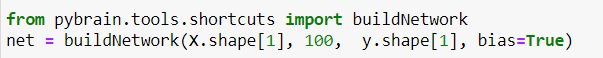
\includegraphics[width=.8\linewidth]{35..png}
\caption{\label{fig:demo-bad}
\centering
\\We import the buildNetwork function and tell it to build a network based on our
necessary dimensions. The first value, X.shape[1], is the number of neurons in the
input layer and it is set to the number of features (which is the number of columns in
X). The second feature is our decided value of 100 neurons in the hidden layer. The
third value is the number of outputs, which is based on the shape of the target array
y. Finally, we set network to use a bias neuron to each layer except  output
layer.}
\end{figure}

\subsection{Assignment 6 (``Back Propagation'')}

\begin{t}
From here, we can now train the network and determine good values for the weights. Starting from the output layer, we compute which neurons were incorrect in their prediction, and adjust the weights into those neurons by a small amount to attempt to fix the incorrect prediction. The process starts at the output layer and goes back each layer until we reach the input layer. At this point, the weights on all connections have been updated. PyBrain contains an implementation of the backprop algorithm, which is called on the neural network through a trainer class.
\end{t}

\begin{figure}[h]
    \centering
    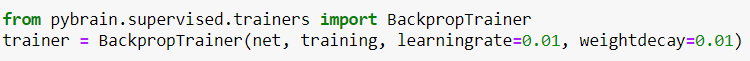
\includegraphics[width=.9\linewidth]{36..png}
\caption{\label{fig:demo-bad}
\centering
\\The backprop algorithm is run iteratively using the training dataset, and each time
the weights are adjusted a little. We can stop running backprop when the error
reduces by a very small amount, indicating that the algorithm isn't improving the
error much more and it isn't worth continuing the training.}
\end{figure}

\begin{t}
In theory, we would run the algorithm until the error doesn't change at all. This is called convergence, but in practice this takes a very long time for little gain.
To make it simple we run the algorithm a fixed number of times, called epochs. The higher the number of epochs, the longer the algorithm will take and the better the results will be. We will train for 20 epochs for this code you can see in figure 37), but trying larger values will increase the performance.
\end{t}

\begin{figure}[h]  
    \centering
    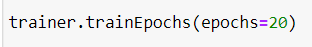
\includegraphics[width=.5\linewidth]{37..png}
\caption{\label{fig:demo-bad}
\centering
epochs\\}
\end{figure}

\newpage
\begin{figure}[h]
    \centering
    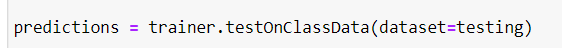
\includegraphics[width=.7\linewidth]{38..png}
\caption{\label{fig:demo-bad}
\centering
\\We can then perform predictions of samples in our testing dataset.}
\end{figure}

\begin{figure}[h]
    \centering
    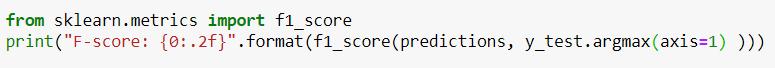
\includegraphics[width=.8\linewidth]{39..png}
\caption{\label{fig:demo-bad}
\centering
\\From these predictions, we can use scikit learn to compute the F1 score.}
\end{figure}

\begin{t}
The score here is 0.97.
\end{t}

\subsection{Assignment 7 (``Predicting Words'')}

\begin{t}
We want to predict each letter from each of these segments, and put those
predictions together to form the predicted word from a given CAPTCHA.
\end{t}

\begin{figure}[h]
    \centering
    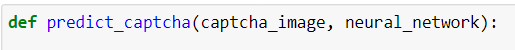
\includegraphics[width=.6\linewidth]{40..png}
\caption{\label{fig:demo-bad}
\centering
\\Our function will accept a CAPTCHA and the trained neural network, and it will return  predicted word.}
\end{figure}

\begin{figure}[hb!]
    \centering
    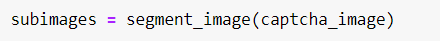
\includegraphics[width=.6\linewidth]{41..png}
\caption{\label{fig:demo-bad}
\centering
\\We extract the sub-images using the segment image function we created earlier.}
\end{figure}

\begin{figure}[hb!]
    \centering
    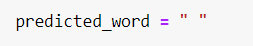
\includegraphics[width=.3\linewidth]{42..png}
\caption{\label{fig:demo-bad}
\centering
\\We will be building our word from each of the letters. The sub-images are ordered
according to their location, so usually this will place the letters in the correct order.}
\end{figure}

\newpage


\begin{figure}[h]
    \centering
    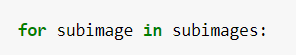
\includegraphics[width=.3\linewidth]{43..png}
\caption{\label{fig:demo-bad}
\centering
iteration\\We iterate over the sub-images}
\end{figure}

\begin{figure}[h]
    \centering
    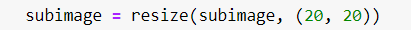
\includegraphics[width=.5\linewidth]{44..png}
\caption{\label{fig:demo-bad}
\centering
\\Each sub-image is unlikely to be exactly 20 pixels by 20 pixels, so we will need to resize it in order to have the correct size for our neural network.}
\end{figure}

\begin{figure}[h]
    \centering
    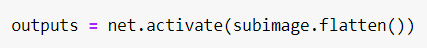
\includegraphics[width=.5\linewidth]{45..png}
\caption{\label{fig:demo-bad}
\centering
\\We will activate our neural network by sending the sub-image data into the input
layer. This propagates through our neural network and returns the given output.}
\end{figure}

\begin{t}
The output of the neural network is 26 numbers, each relative to the likelihood that
the letter at the given index is the predicted letter. To get the actual prediction, we
get the index of the maximum value of these outputs and look up our letters list
from before for the actual letter. For example, if the value is highest for the fifth
output, the predicted letter will be E. Ypo can see in fig 46
\end{t}

\begin{figure}[hb!]
    \centering
    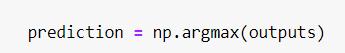
\includegraphics[width=.4\linewidth]{46..png}
\caption{\label{fig:demo-bad}
\\}
\end{figure}

\begin{figure}[hb!]
    \centering
    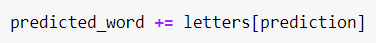
\includegraphics[width=.5\linewidth]{47..png}
\caption{\label{fig:demo-bad}
\centering
\\We then append the predicted letter to the predicted word we are building}
\end{figure}


\begin{figure}[hb!]
    \centering
    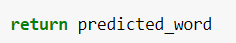
\includegraphics[width=.3\linewidth]{48..png}
\caption{\label{fig:demo-bad}
\centering
\\After the loop completes we have go through each of the letters and formed our predicted word. }
\end{figure}

\newpage
\begin{figure}[h]   
    \centering
    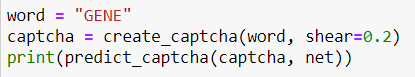
\includegraphics[width=.5\linewidth]{49..png}
\caption{\label{fig:demo-bad}
\centering
\\We tested on a word. }
\end{figure}

\begin{figure}[h]
    \centering
    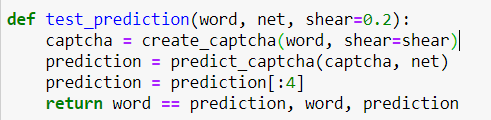
\includegraphics[width=.7\linewidth]{50..png}
\caption{\label{fig:demo-bad}
\centering
\\We coded this testing into function. }
\end{figure}

\begin{t}
This code correctly predicts the word GENE, but makes mistakes with other words. To test the accuracy we will create a dataset with a whole bunch of four-letter English words from NLTK as you can see in fig 51:
\end{t}

\begin{figure}[h]
    \centering
    \includegraphics[width=.5\linewidth]{51..png}
\caption{\label{fig:demo-bad}
\\ }
\end{figure}

\begin{figure}[hb!]
    \centering
    \includegraphics[width=.9\linewidth]{52..png}
\caption{\label{fig:demo-bad}
\centering
\\The words instance here is actually a corpus object, so we need to call words() on it
to extract the individual words from this corpus. We also filter to get only four letter
words from this list. }
\end{figure}

\newpage
\begin{figure}[hb!]
    \centering
    \includegraphics[width=.8\linewidth]{53..png}
\caption{\label{fig:demo-bad}
\centering
\\We can then iterate over all of the words to see how many we get correct by simply
counting the correct and incorrect predictions. }
\end{figure}

\begin{t}
The results we get are 2,832 correct and 2,681 incorrect for an accuracy of just over
51 percent. But we had 0.97 above. The first factor to impact is our accuracy. All other things being equal, if we have four letters, and 97 percent accuracy per-letter, then we can expect about an 88 percent success rate getting four letters in a row (0.880-0.974). A single error in a single letter's prediction results in the wrong word being predicted.
The second impact is the shear value. Our dataset chose randomly between shear
values of 0 to 0.5. The previous test used a shear of 0.2. For a value of 0, we get 75
percent accuracy; for a shear of 0.5, the result is much worse at 2.5 percent. The
higher the shear, the lower the performance.
The next impact is that our letters were randomly chosen for the dataset. Letters, such as E, appear much more frequently than other letters, such as Q. Letters that appear reasonably commonly but are frequently mistaken for each other, will also contribute to the error.
We can table which letters are frequently mistaken for each other using a confusion
matrix, which is a two dimensional array. Its rows and columns each represent an
individual class.
\end{t}

\begin{figure}[hb!]
    \centering
    \includegraphics[width=.8\linewidth]{54..png}
\caption{\label{fig:demo-bad}
\centering
\\Each cell represents the number of times that a sample is actually from one class
(represented by the row) and predicted to be in the second class (represented by
the column). For example, if the value of the cell (4,2) is 6, it means that there were
six cases where a sample with the letter D was predicted as being a letter B. }
\end{figure}

\begin{t}
Ideally, a confusion matrix should only have values along the diagonal. The cells (i, i)
have values, but any other cell has a value of zero. This indicates that the predicted classes
are exactly the same as the actual classes. Values that aren't on the diagonal represent errors in the classification.
\end{t}

\begin{figure}[ht]
    \centering
    \includegraphics[width=.4\linewidth]{55..png}
\caption{\label{fig:demo-bad}
\centering
\\We can also plot this using pyplot, showing graphically which letters are confused
with each other. }
\end{figure}

\newpage
\begin{figure}[h]
    \centering
    \includegraphics[width=.5\linewidth]{56..png}
\caption{\label{fig:demo-bad}
\centering
\\We set the axis and tick marks to easily reference the letters each index
corresponds to. }
\end{figure}

\begin{figure}[hb!]
    \centering
    \includegraphics[width=.8\linewidth]{aradaki graph.png}
\caption{\label{fig:demo-bad}
\centering
\\The result is shown in the next graph. It can be quite clearly seen that the main
source of error is U being mistaken for an H nearly every single time. The letter U appears in 17 percent of words in our list. For each word that a U appears in, we can expect this to be wrong. U actually appears more often than H (which is in around 11 percent of words), indicating we could get a cheap (although possibly not a robust) boost in accuracy by changing any H prediction into a U }
\end{figure}

\newpage
\subsection{Assignment 8 (``Ranking Mechanisms For Words'')}

\begin{t}
The Levenshtein edit distance is a commonly used method for comparing two short
strings to see how similar they are. It isn't very scalable, so it isn't commonly used for
very long strings. The edit distance computes the number of steps it takes to go from
one word to another. The steps can be one of the following three actions:
1. Insert a new letter into the word at any position.
2. Delete any letter from the word.
3. Substitute a letter for another one.
The minimum number of actions needed to transform the first word into the second
is given as the distance. Higher values indicate that the words are less similar
\end{t}

\begin{figure}[h]
    \centering
    \includegraphics[width=.7\linewidth]{57..png}
\caption{\label{fig:demo-bad}
\centering
\\This distance is available in NLTK as nltk.metrics.edit-distance. We can call
it using on two strings and it returns the edit distance }
\end{figure}

\begin{t}
 At this point we don't really expect letters to be moved around, just
individual letter comparisons to be wrong. For this reason, we will create a different
distance metric, which is simply the number of letters in the same positions that are
incorrect. 
\end{t}

\begin{figure}[h]
    \includegraphics[width=.8\linewidth]{58..png}
    \centering
\caption{\label{fig:demo-bad}
\centering
\\We subtract the value from the length of the prediction word (which is four) to make
it a distance metric where lower values indicate more similarity between the words. }
\end{figure}

\subsection{Assignment 9 (``Putting It All Together'')}

We can now test our improved prediction function using similar code to before.

\begin{figure}[hb!]
    \centering
    \includegraphics[width=.7\linewidth]{59..png}
\caption{\label{fig:demo-bad}
\centering
\\First we define a prediction, which also takes our list of valid words. }
\end{figure}

\newpage
\begin{t}
We do our prediction and limit it to the first four characters. We now check if the word is in the dictionary or not. If it is, we return that as our prediction. If it is not, we find the next nearest word.
\end{t}

\begin{figure}[h]
    \centering
    \includegraphics[width=.5\linewidth]{60..png}
\caption{\label{fig:demo-bad}
\\ }
\end{figure}

\begin{figure}[hb!]
    \centering
    \includegraphics[width=.7\linewidth]{61..png}
\caption{\label{fig:demo-bad}
\centering
\\ We compute the distance between our predicted word and each other word in the
dictionary, and sort it by distance (lowest first).}
\end{figure}

\begin{figure}[h]
    \centering
    \includegraphics[width=.5\linewidth]{62..png}
\caption{\label{fig:demo-bad}
\centering
\\We then get the best matching word, the one with the lowest distance and
predict that word. }
\end{figure}

\begin{figure}[hb!]
    \centering
    \includegraphics[width=.6\linewidth]{63..png}
\caption{\label{fig:demo-bad}
\centering
\\ We then return the correctness, the word, and prediction.}
\end{figure}


\begin{figure}[hb!]
    \centering
    \includegraphics[width=.9\linewidth]{64..png}
\caption{\label{fig:demo-bad}
\centering
\\The changes of code in fig 53.}
\end{figure}

\newpage
\begin{t}
The preceding code will take a while to run (computing all of the distances takes
some time) but the net result is 3,037 samples correct and 2,476 samples incorrect.
This is an accuracy of 55 percent for a boost of 4 percentage points. The reason this
improvement is so low is that multiple words all have the same similarity, and the
algorithm is choosing the best one randomly between this set of most similar words.
For example, the first word in the list, AANI has 44 candidate words that
are all the same distance from the word. This gives just a 1/44 chance of choosing
the correct word from this list.
\end{t}

\section{Conclusion}
In this project we worked with images in order to use simple pixel values to
predict the letter in a CAPTCHA. We only used complete four letter English words. We created our own dataset of CAPTCHAs and letters, used scikit image library to work with images data, we used PyBrain library for neural networks, we extracted basic features from images. We were able to create a feed-forward neural network to accurately predict which letter was in the image. At this stage, our results were very good with 97 percent accuracy. We improved our accuracy using a dictionary, searching for the best matching word. To do this, we considered the commonly used edit distance.\\
With this project we had a chance work with different libraries, modules and we had a chance to gain more experiences. 






\end{document}